
%
%   svt_calibrations.tex
%       author: Omar Moreno <omoreno1@ucsc.edu>
%               Per Hansson <phansson@slac.stanford.edu>
%      created: November 13, 2012
%

In order to prepare the SVT for real physics data-taking, the SVT was 
calibrated. This involved the extraction of the mean baseline (pedestal),
noise and gain for each of the 12,780 SVT channels. All measurements
were made with the APV25 readout chips configured to their nominal operating
points \cite{Jones:1069892} and all sensors biased to 180 V. The APV25s were
operated in ``multi-peak'' mode with six samples being readout per trigger.
This, in turn, allowed for the extraction of the $t_0$ and amplitude of the 
signals being read out.

Figure~\ref{fig:pedestal_noise} shows an intensity plot of the pedestals 
along with the readout noise as a function of channel number for a single
hybrid.  The noise was computed by taking the RMS of the Gaussian distributed
\begin{figure}[h]
    \begin{center}
    	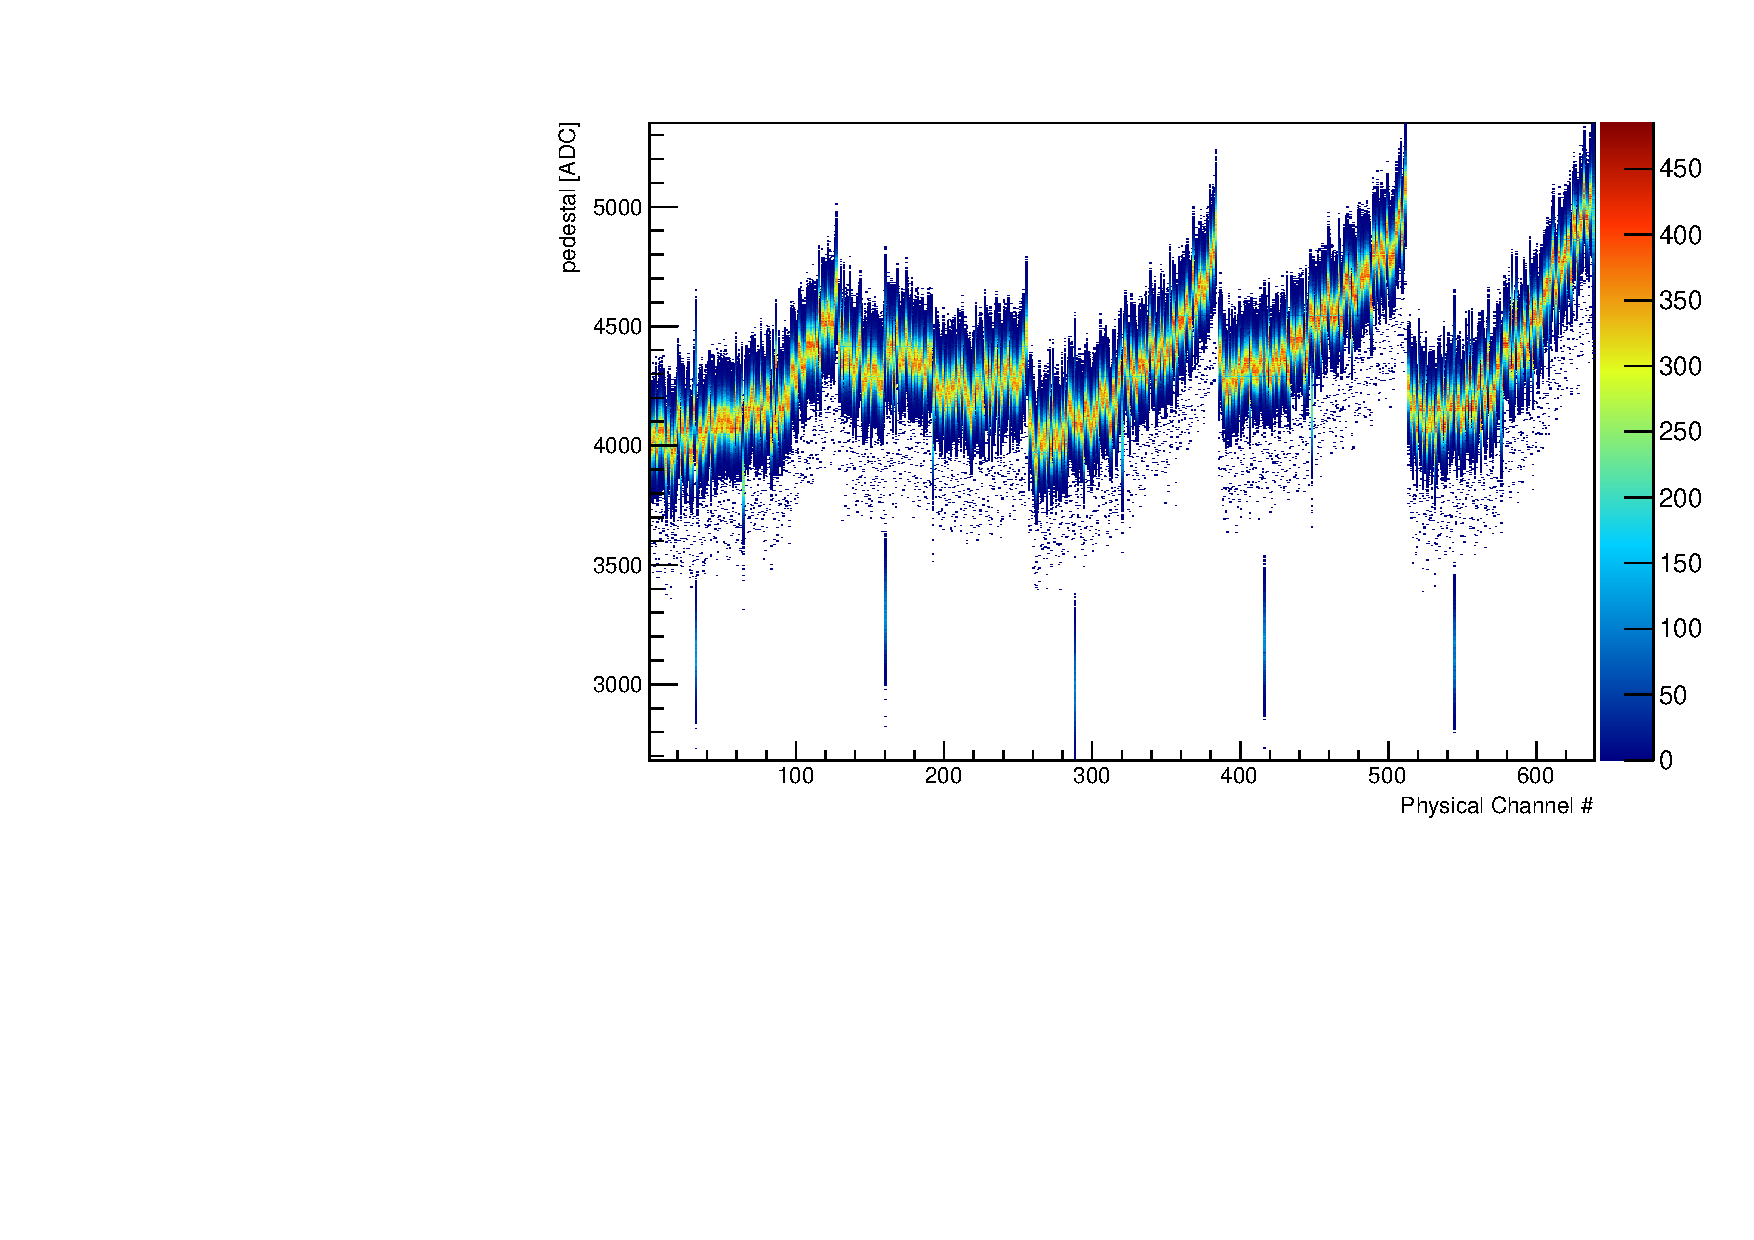
\includegraphics[width=0.49\textwidth]{test2012/svtperformance/svt_calib/baseline_v_ch_fpga0_hybrid0.pdf}
    	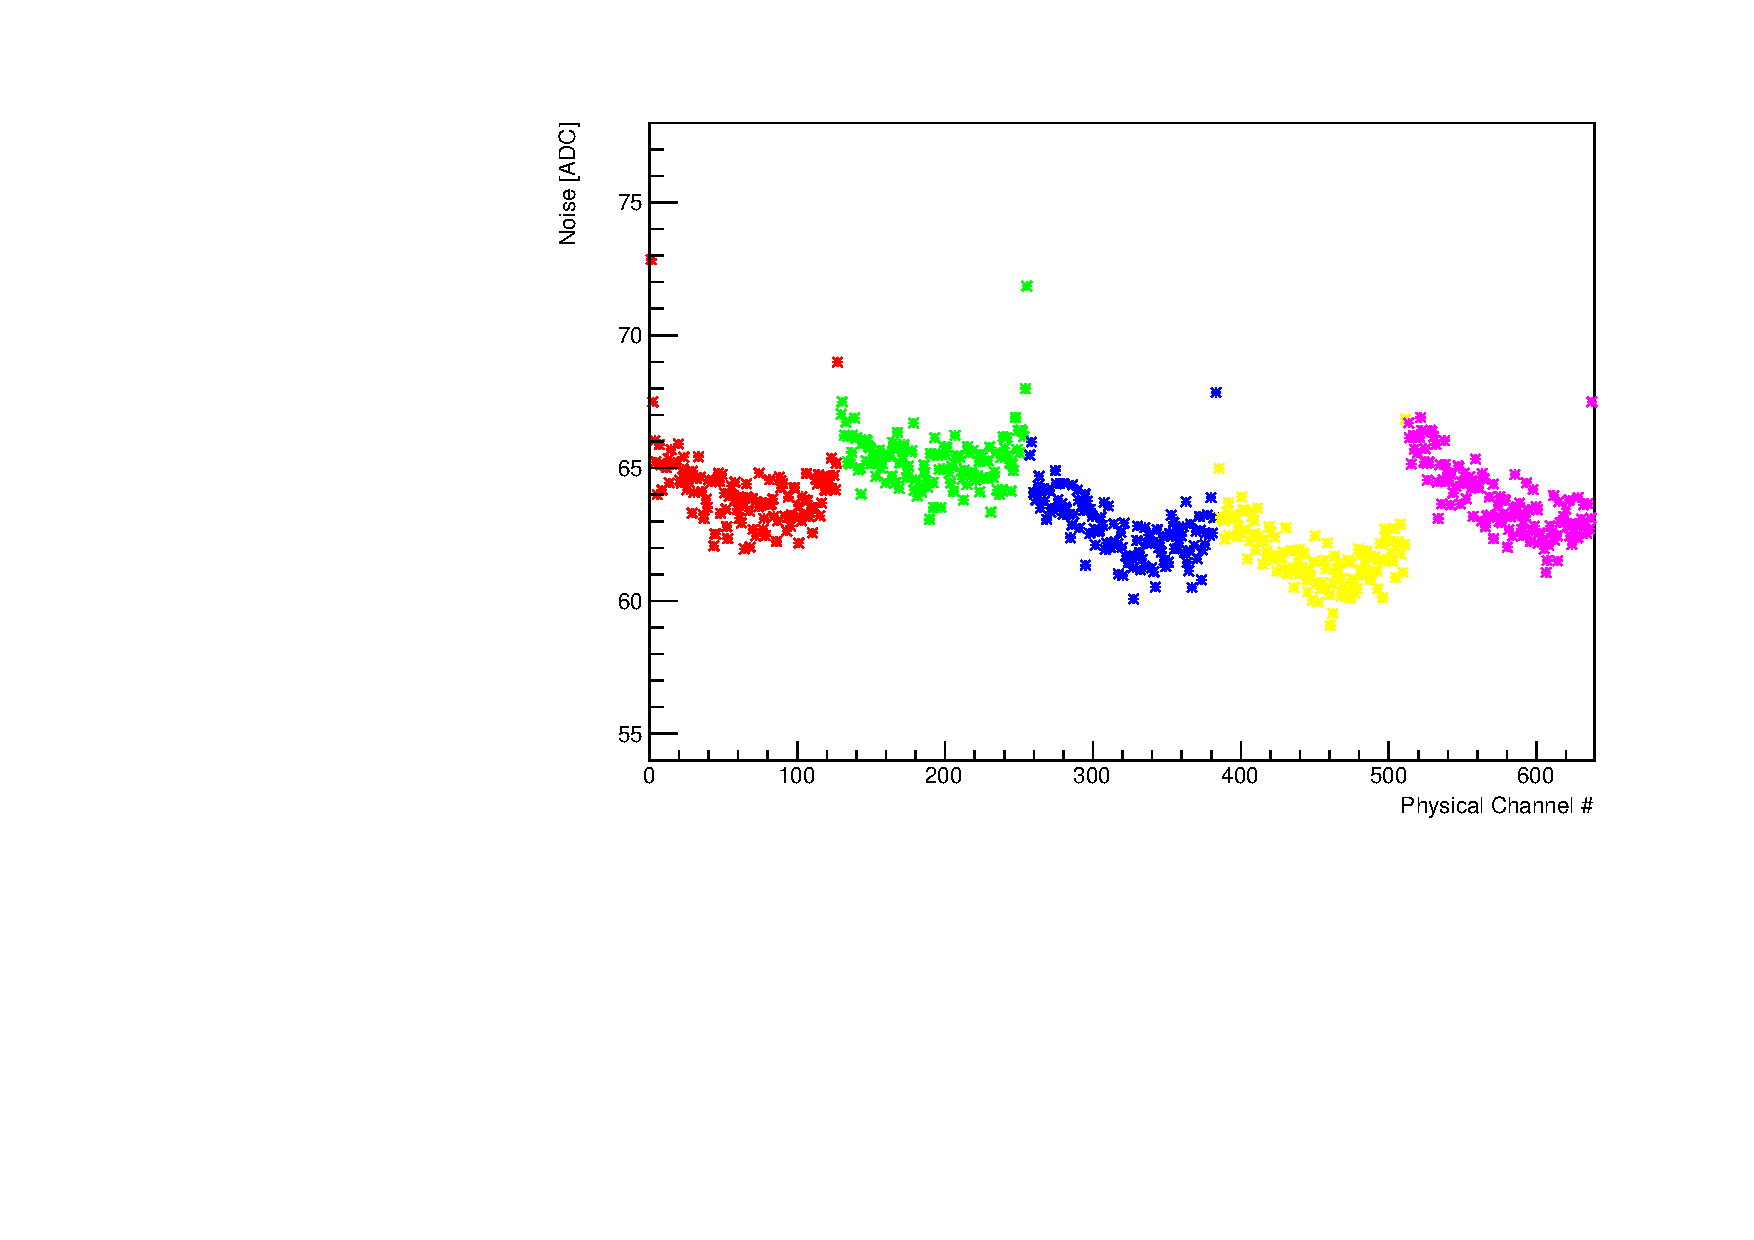
\includegraphics[width=0.49\textwidth]{test2012/svtperformance/svt_calib/noise_v_ch_fpga0_hybrid0_0.pdf}
        \caption{The baseline distributions for a single hybrid are shown on
                 the left plot. The overall baseline shifts were calibrated 
                 out. The measured noise is shown on the right with the 
                 different colors denoting a different APV25 readout chip.  
                 The large noise values at the chip edges have also been 
                 observed by the CMS collaboration and the cause is still 
                 under investigation.
                 } 
	\label{fig:pedestal_noise}
    \end{center}
\end{figure}
pedestals for each of the channels and was observed to be consistently within 
60 - 68 ADC counts ($\approx$ 667 - 756 electrons).  
Figure~\ref{fig:pedestal_noise} also demonstrates a feature common amongst 
all APV25 readout chips, mainly the large values of noise for channels 
lying near the chip edges.  This was also  observed by the CMS 
collaboration and the cause is still under investigation.

Another aspect which is crucial to full characterization of the SVT is an 
understanding of the signal response and the associated gain.
Using the APV25 internal calibration circuitry, a known fixed charge was 
injected into all channels.  This allowed for the accurate determination
of the signal response along with its scaling with input charge.
\begin{figure}[h]
    \begin{center}
        % TODO: Both of these plots need to be remade.  The current plots
        % will serve as place holders for now.
        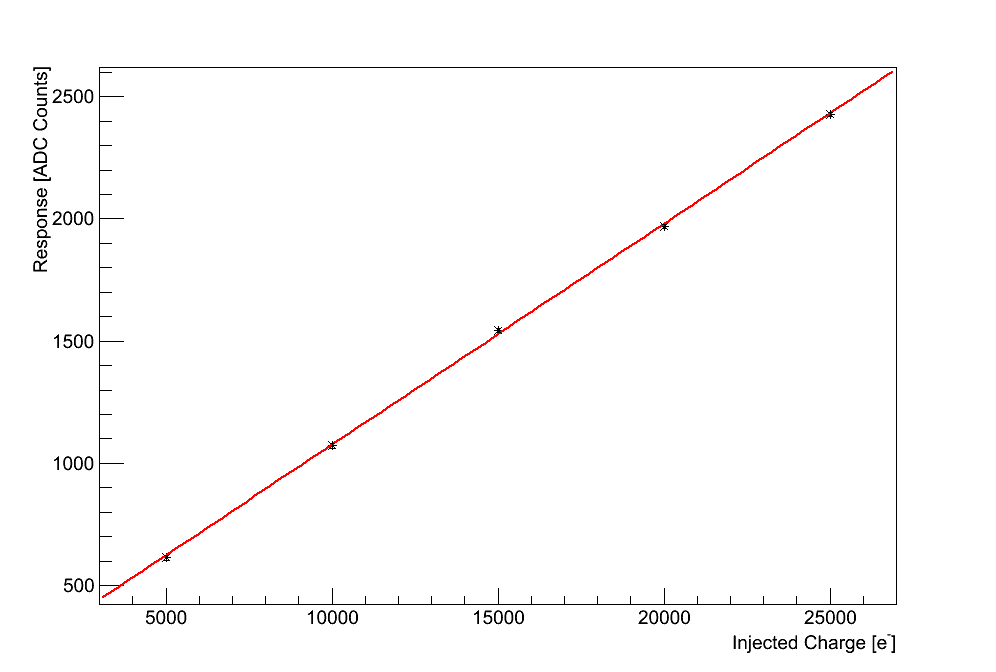
\includegraphics[width=0.49\textwidth]{test2012/svtperformance/svt_calib/response_curve_fpga0_hybrid0_channel0.png}
        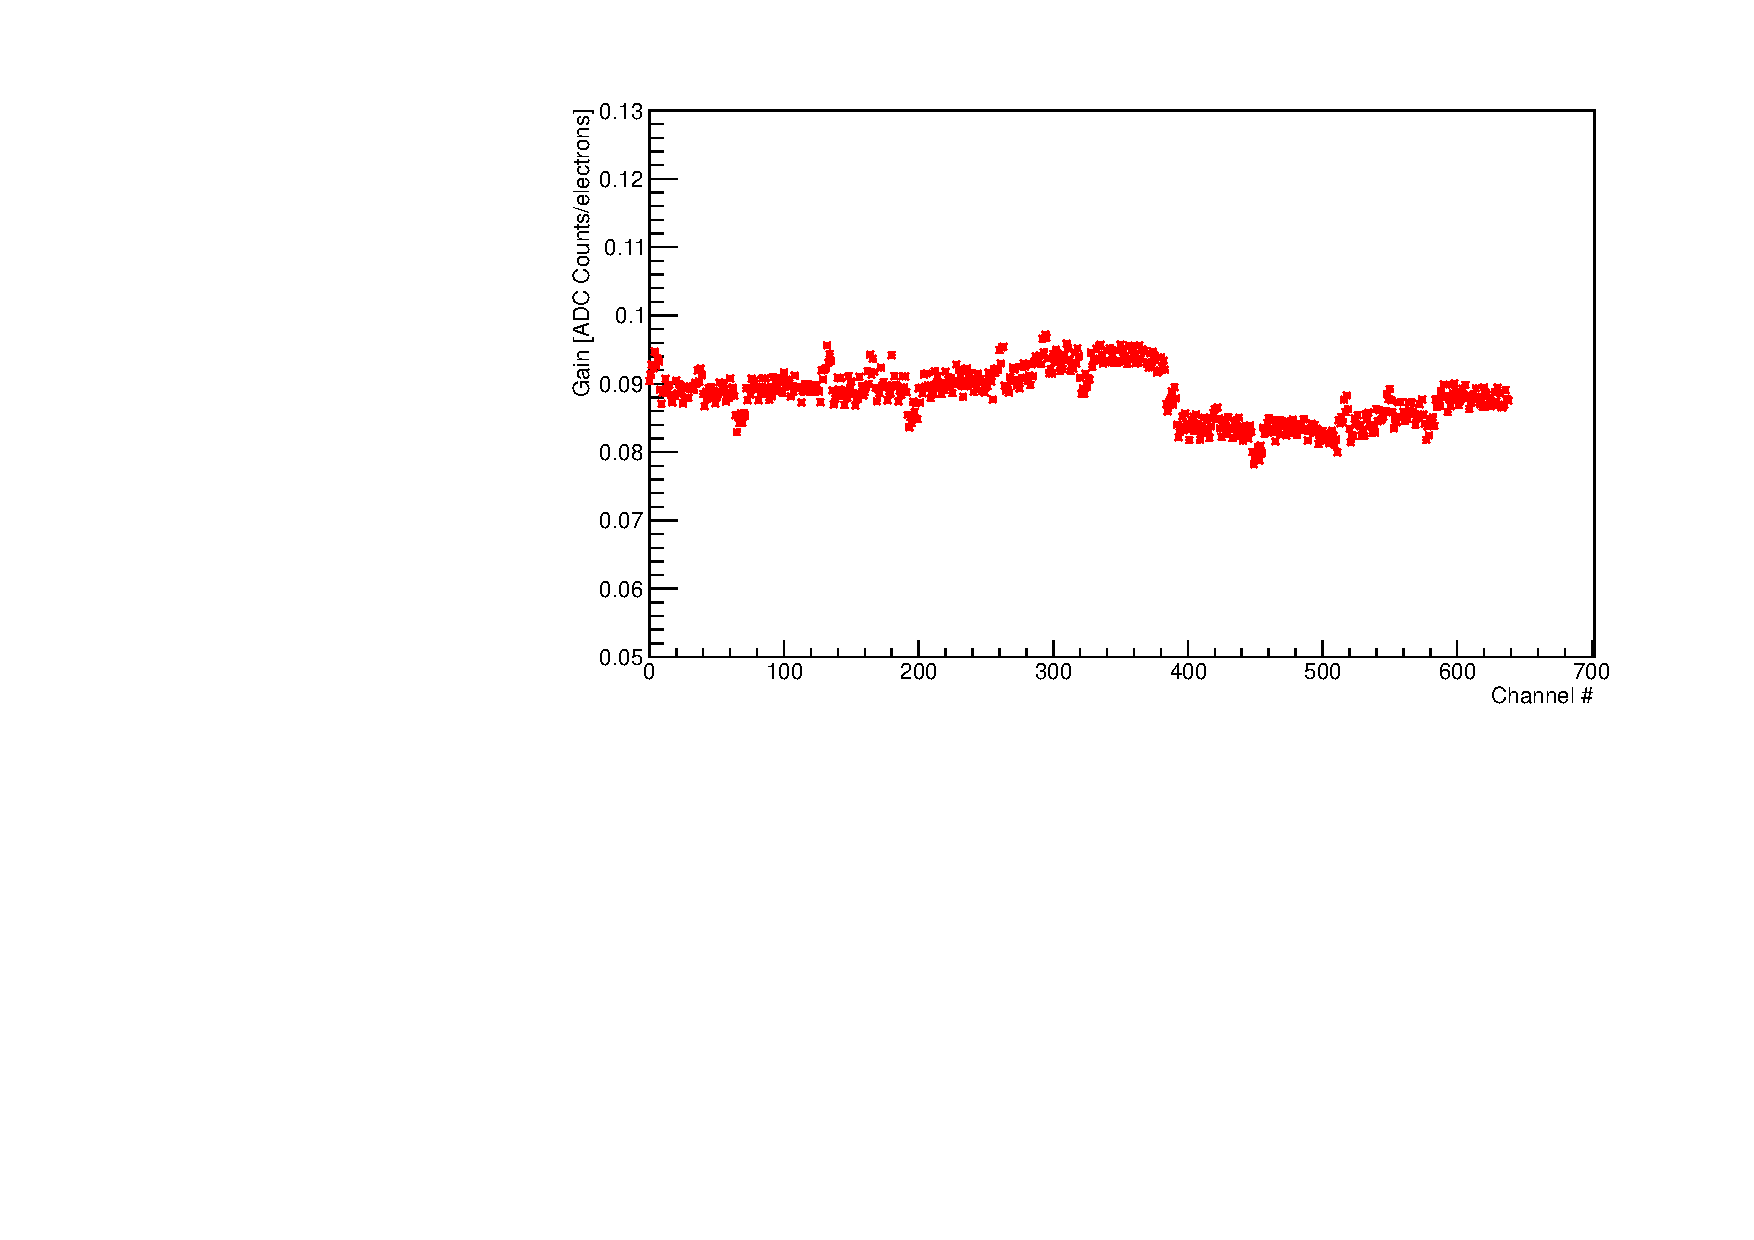
\includegraphics[width=0.49\textwidth]{test2012/svtperformance/svt_calib/gain_stability_fpga0_hybrid0.pdf}
        \caption{Fit of the signal response as a function of charge over a 
                 range of 0 to 25,000 electrons is shown on the left plot.
                 The response shows good linearity up to $\approx$ 3 MIPs. The
                 gain uniformity, shown on the right, was within the expected
                 range across all chips.
                }
        \label{fig:gain} 
    \end{center}
\end{figure}
As shown on Figure~\ref{fig:gain}, the response exhibits good linearity up 
to $\approx$ 3 MIPs while the gain uniformity was within the expected range 
across all chips on a hybrid.

All reconstructed hits in an event were used to form clusters of energy 
depositions using a nearest neighbor algorithm. Figure~\ref{fig:cluster_pulse}
shows the mean pulse shape of each of the hits associated with a track as a 
function of time.  
\begin{figure}[h]
    % TODO: The pulse plot needs to be remade such that the x-axis is time 
	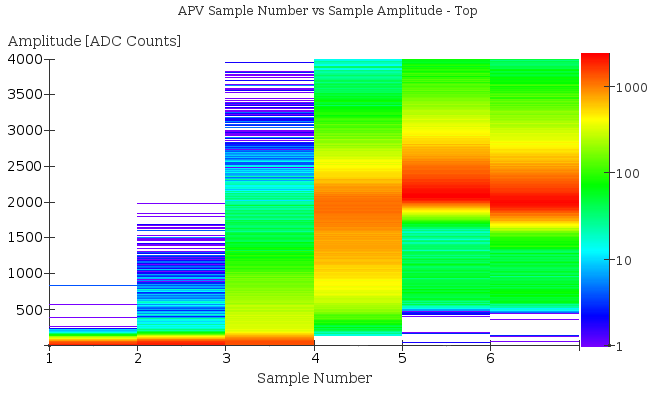
\includegraphics[width=0.49\textwidth]{test2012/svtperformance/svt_calib/08062012_run1351_samples_vs_amplitude.png}
	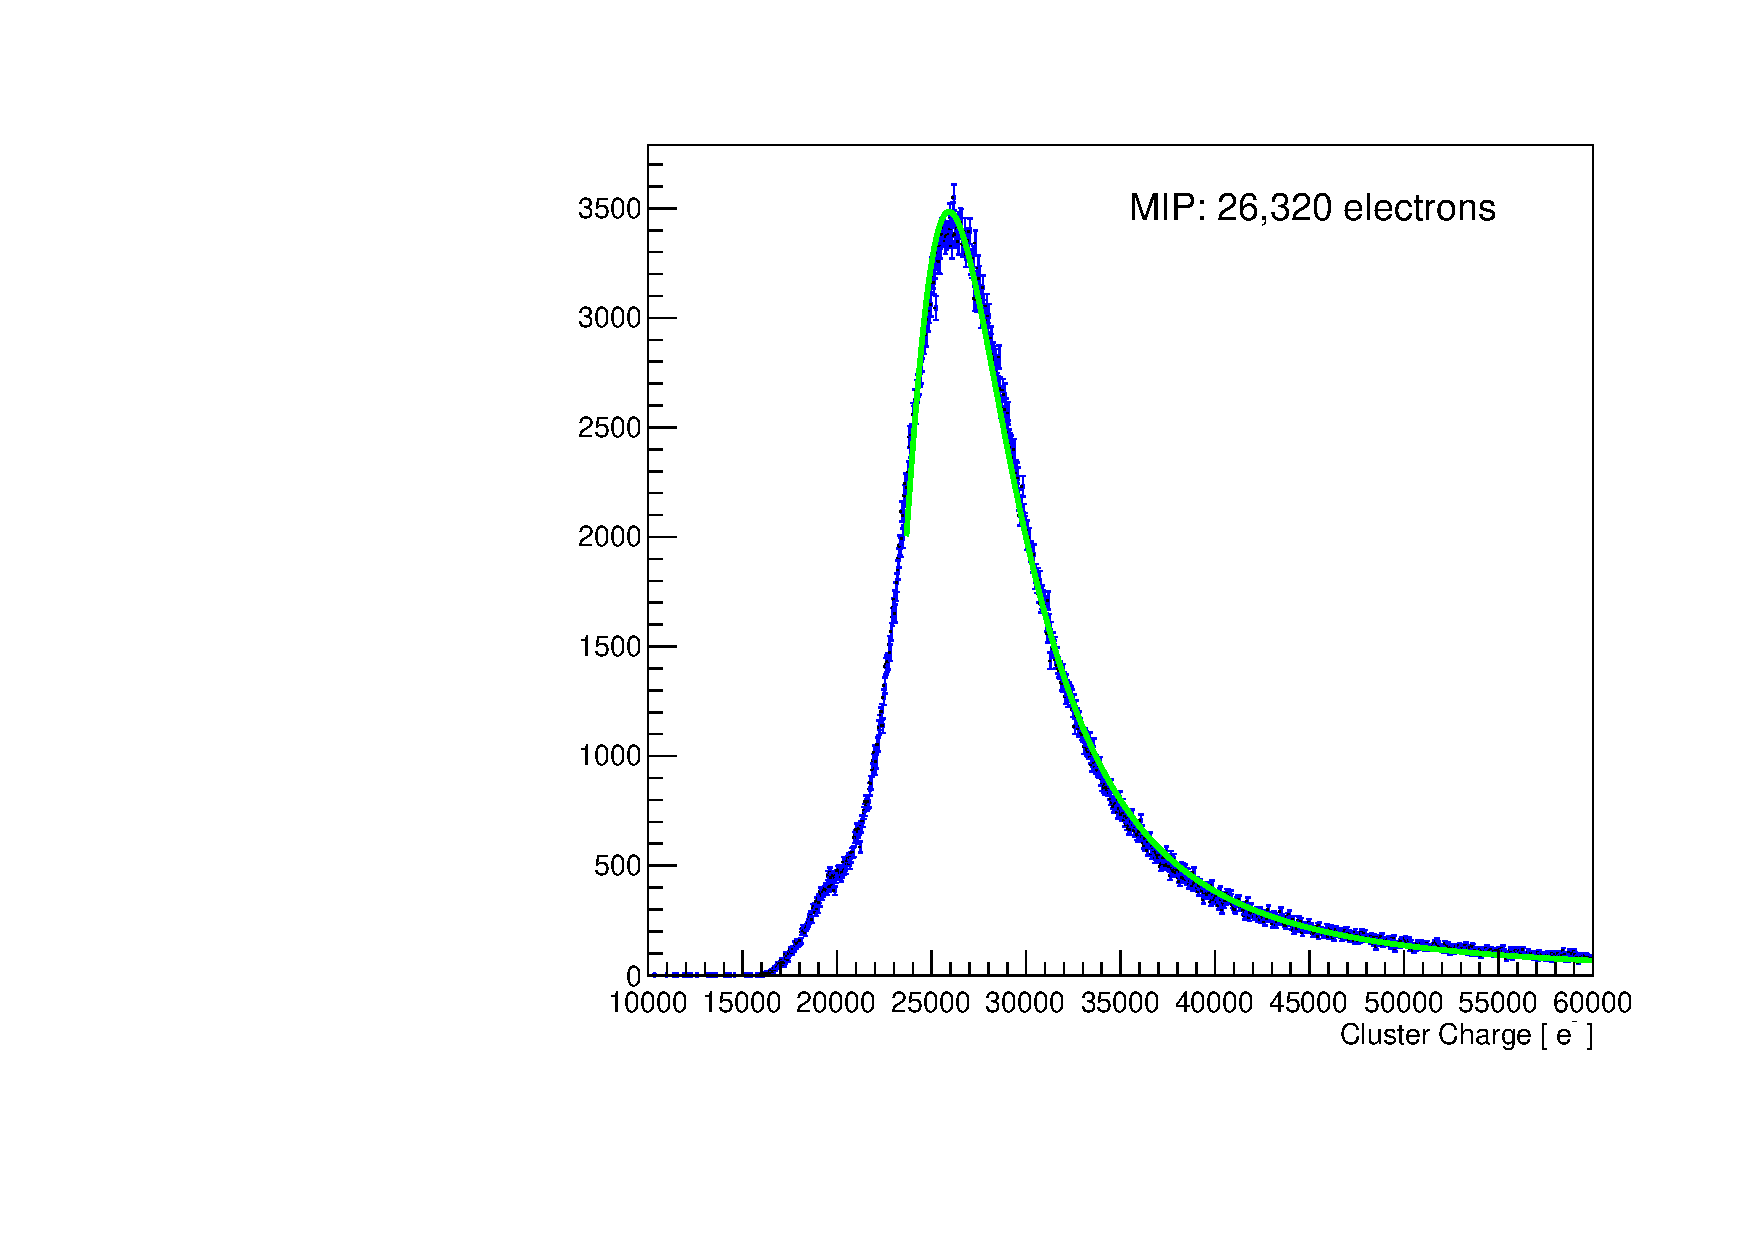
\includegraphics[width=0.49\textwidth]{test2012/svtperformance/svt_calib/run1351_mip_small.pdf}
    \caption{The six pedestal subtracted samples associated with a hit on a track 
             are shown on the left plot along with a distribution of the cluster
             charge exhibiting the characteristic Landau shape on the right. 
            }
	\label{fig:cluster_pulse}
\end{figure}
The figure also demonstrates that  the trigger system, described below, was well 
timed in with the tracker. Figure~\ref{fig:cluster_pulse} also shows the MIP 
% The MIP value seems small ... going to look at the gains again at some point
response to be 14,128 electrons. This yields a signal to noise ratio
of 25.5 which is well matched to the value expected from first principles.

\bibliography{svt_calib}
 
